%\documentclass[wcp,gray]{jmlr} % test grayscale version
\documentclass[wcp]{jmlr}

% Loaded automatically: amsmath, amssymb, natbib, graphicx, url, algorithm2e
\usepackage{booktabs}
\usepackage{pifont}

% Do not comment the following commands:
\pagenumbering{gobble}
\newcommand{\cs}[1]{\texttt{\char`\\#1}}
\makeatletter
\let\Ginclude@graphics\@org@Ginclude@graphics
\makeatother

\jmlryear{2026}
\jmlrworkshop{ACML 2026 Workshop: AMIW}

\title[Composing Pansori Without a Melody Model]{Plan, Then Sing: Composing Pansori
Without a Melody Model}

\author{\Name{Anonymous Author} \Email{}\\ \addr Anonymous Institution}

\editors{Andy Song, Bo Han and Sarah Erfani}

\begin{document}

\makeatletter
\let \@jmlrpages \@empty
\makeatother

\maketitle

\begin{abstract}
Pansori, the Korean tradition of solo narrative singing, survives only as recordings, with
no scores and no aligned lyrics. We describe how 394 commercial recordings became a
singing-voice synthesis (SVS) model and a composition tool, and the measurement behind each
step. A speech aligner hears 52.2\% of corpus time as silence where the singer holds a
note even at 6\,s; a fine-tuned singing aligner cuts the share of phones at the 30\,ms floor from
26.4\% to 2.7\%. Snapping transcripts to the published libretto made a trained model worse;
borrowing only its spelling, at the sung syllable count, did not. The model reproduces how
much the voice moves inside a note but not where, so the tool retrieves note skeletons from
14,244 corpus phrases and lets the user rebind the syllables. On 125 held-out passages, its
unedited output lies at a kernel audio distance of 15.4 from the recordings, against 43.3
for a general song model and 0.27 between halves of the recordings.
\end{abstract}
\begin{keywords}
pansori; singing voice synthesis; low-resource music; forced alignment;
human-AI co-creation
\end{keywords}

%==============================================================================
\section{Introduction}
%==============================================================================
In \emph{pansori}, one singer and one drummer perform a story that can run for hours.
The voice is deliberately rough, and its long sustained tones carry \emph{sigimsae}:
bends, shakes and slides that travel a semitone or more around the nominal note.
Melodies are organized by mode (\emph{akjo}: \emph{gyemyeonjo}, \emph{ujo},
\emph{pyeongjo}) and by rhythmic cycle (\emph{jangdan}). Composing a new passage, called
\emph{jakchang}, means fitting a text to a mode and deciding \emph{butimsae}, the
placement of syllables against the melody and the rhythmic cycle.

An SVS model needs recordings with time-aligned phonemes and notes, and pansori has
neither. Every label comes from a tool built for other material (separator, speech
recognizer, note transcriber, aligner), each fails on pansori in its own way, and most of
the work lies in measuring where. Even then there are no scores to sing from, and
lyrics-to-melody models count beats and stay inside a scale. So the tool retrieves
melodies from real phrases, a person edits how the lyrics bind to them, and the model
supplies the ornament. We contribute:
\begin{itemize}
  \item a pipeline from recordings to a pansori SVS corpus, with the measurement behind
    each decision: utterance length, aligner and lyric source;
  \item a plan-then-render composition tool that needs no melody model;
  \item a set-level measurement of how close the tool's unedited output sounds to held-out
    recordings.
\end{itemize}

%==============================================================================
\section{Related Work}
%==============================================================================
Lyrics-to-melody generation has moved from sequence-to-sequence pre-training with
syllable--note alignment \citep{sheng2021songmass} to template-based two-stage systems
that pass through rhythm, chord and cadence \citep{ju2022telemelody}, and to decoding
constrained by lyric--melody relationships \citep{zhang2022relyme}. All three count
duration in beats and treat a syllable over several notes as the exception; here 42.2\% of
syllables carry more than one note, and GaMaDHaNi models Hindustani singing as a pitch
contour for that reason \citep{shikarpur2024gamadhani}. Cococo
restricted generation to parts of a piece so as not to overwhelm novices
\citep{louie2020cococo}; our tool takes the same stance. General song models such as
ACE-Step \citep{gong2026acestep} sing lyrics in a style named by a caption; we use one to
calibrate our measurement.

%==============================================================================
\section{From Recordings to a Singing Model}\label{sec:pipeline}
%==============================================================================
\textbf{Corpus.} The source is 394 commercial recordings with vocals separated by HT-Demucs
\citep{rouard2023htdemucs}; section labels mark each sung span's mode, and spoken
(\emph{aniri}) spans are excluded. Whisper large-v3 \citep{radford2023whisper} transcribes
the lyrics, with repeated syllables collapsed because a held tone sounds to it like one
syllable sung many times. ROSVOT \citep{li2024rosvot} transcribes the notes.

\textbf{Utterances of at most 6\,s.} The Korean model of MFA \citep{mcauliffe2017mfa} was
trained on speech and gives up on long held tones: on a small sample, utterances over 6\,s
averaged 4.06\,s of aligned silence and those under 6\,s had no silence of 1\,s or more.
We cut at pauses of 0.4\,s or more (p90 of all pauses is 0.66\,s; shorter ones lie mostly
inside \emph{sigimsae}), and cut a pauseless melisma at the widest gap between its
notes, never inside a held tone: 31,529 utterances (33.48\,h) of 2 to 6\,s.

\textbf{Why SOFA.} Even at 6\,s, MFA leaves 26.4\% of phones at 30\,ms or less, boundaries
it declined to place, and labels 52.2\% of corpus time as silence while a note covers it: a
sustained tone, not a rest. We absorb such silence into the preceding phone, and replace
the aligner with SOFA \citep{sofa}, which is built for singing. It has no Korean checkpoint,
so we fine-tune its multilingual singing checkpoint with a new head for Korean phonemes, on
labels bootstrapped from MFA. Given every MFA timing, SOFA learns the floor too, so timings
are kept only for utterances with at most 15\% of phones at the floor (4,501); the other
22,454 contribute their phoneme sequence alone. A second round, bootstrapped from the first
SOFA's alignment, trusts 11,498. The final corpus (26,955 utterances, 28.93\,h, 23 singers)
has 2.7\% of phones at 30\,ms or less, and its median phone grows from 80 to 157\,ms.

\textbf{Lyrics against the libretto.} Whisper mishears archaic Sino-Korean, and every piece
has a published libretto (\emph{changbon}). Matched without the piece's name, the chosen
libretto agreed with it for all 295 recordings past a confidence gate, and 11,174 of 31,529 segments
were rewritten. The rewrites were mostly right, yet a model trained on them lost
voiced/unvoiced agreement where the lyrics had changed, 21 items to 6 (sign test
$p{=}0.006$; unchanged controls 10 to 12). Where the match was weak, the libretto span ran
to twice the sung syllable count at p90, and such a label is wrong however it is spelled.
The \emph{hybrid} text keeps Whisper's syllables one for one and borrows libretto
syllables only over equal-length stretches pinned by exact matches (22.2\% of syllables in
matched segments). Against Whisper's text, each with its own aligner, none of nine sign
tests reached $p{<}0.05$ (60 held-out pairs $\times$ 3 seeds); we keep the canonical
spelling.

\textbf{Training.} Our earlier model, a FastSpeech2-style cascade at 24\,kHz, copied a vowel
once per note it spanned. In the openvpi fork \citep{openvpi} of DiffSinger
\citep{liu2022diffsinger}, notes keep their own time axis, so \emph{sigimsae} is just
several notes over one syllable, and a dictionary of all 11,172 Hangul syllables lets the
model sing unseen text. Public checkpoints use a Mandarin phoneme set, so a variance model
(25.1\,M parameters; durations and f0) and an acoustic model (69.1\,M; mel) are trained
from scratch with rectified flow \citep{liu2023flow}, with f0 extracted by RMVPE
\citep{wei2023rmvpe} over 55--750\,Hz (the default 65\,Hz floor silences the male low
register) and an NSF-HiFiGAN vocoder \citep{openvpivocoders}. One piece from each of five
singers is held out. Each model runs 40,000 steps on one RTX 4090 (0.9\,h and 0.4\,h), and
each head is taken from its own best validation step (acoustic 32k, duration 28k, pitch
36k); in an earlier run, taking pitch from the total-loss optimum cost 25\% more f0 error.

\textbf{What the engine learns.} On 19 held-out utterances, predicting f0 from the score
with true durations (median of 5 seeds), the ratio of synthesized to recorded within-note
f0 variation rises from the earlier model's 0.29 to 0.95 (95\% CI of the paired difference
$[0.35, 0.68]$, Holm $p{=}0.0003$), but correlation with the recorded contour, 0.04
against 0.16, is not significant (Holm $p{=}0.24$). The engine moves as much as a singer
but not where the singer moves, so the skeleton and binding come from real phrases and the
user.

%==============================================================================
\section{The Composition Tool}
%==============================================================================
\begin{figure}[t]
\centering
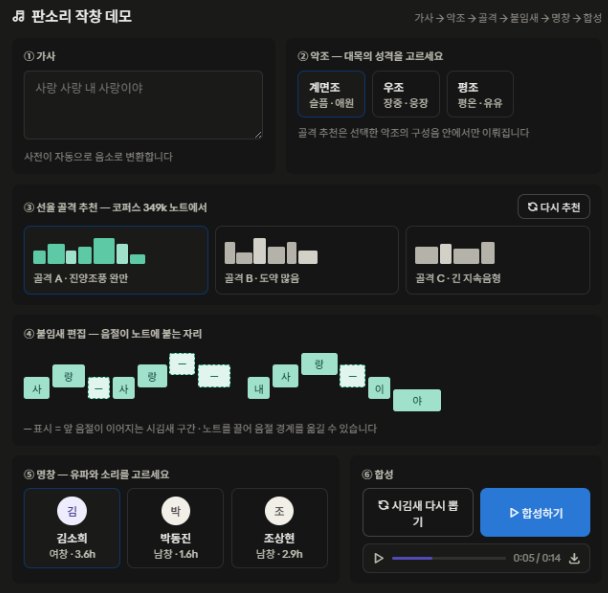
\includegraphics[width=0.38\linewidth]{figs/demo.png}
\caption{The tool (UI in Korean). \ding{172}~lyrics; \ding{173}~mode; \ding{174}~three
retrieved skeletons with measured shape labels; \ding{175}~\emph{butimsae} editor, where
syllable chips are dragged across notes and ``--'' marks a held syllable;
\ding{176}~singer; \ding{177}~render, or redraw the ornamentation.}
\label{fig:demo}
\end{figure}

The tool (Fig.~\ref{fig:demo}) never sings straight from the lyrics: it returns an editable
\emph{plan} of notes, each with a pitch, a duration in seconds and its syllable, and renders
only the plan the user sends back.

\textbf{Skeletons are retrieved.} A monotonic dynamic program binds each aligned syllable
to a contiguous run of notes, and the phrases are indexed by mode: 10,309
\emph{gyemyeonjo}, 3,081 \emph{ujo} and 854 \emph{pyeongjo} skeletons. Each 2--12 syllable
chunk of the user's lyrics is offered three skeletons of the nearest syllable count with
different measured shapes, transposed to the singer's centre and never quantized to a scale.
The mode is in these notes: a linear probe separates \emph{ujo} from \emph{gyemyeonjo}
pitch-class profiles at 72.3\% balanced accuracy, singers held out (51.4\% shuffled).

\textbf{\emph{Butimsae} is edited.} Dragging a syllable chip moves a syllable boundary
while the notes stay fixed. \emph{Render} keeps the seed, so two renders differ only by the
edit; \emph{Redraw} changes only the seed, drawing new ornamentation over the same notes.

%==============================================================================
\section{Does the Output Sound Like Pansori?}\label{sec:kad}
%==============================================================================
\begin{table}[t]
\centering
\small
\caption{Kernel audio distance ($\times 100$) to 125 held-out recordings; lower is closer.
Generated sets mix 3 seeds, and brackets are 95\% bootstrap intervals. The first row is
the distance between two singer-stratified halves of the recordings (mean over 200 splits,
95th percentile in parentheses).}
\label{tab:kad}
\begin{tabular}{lcc}
\toprule
 & CLAP & MERT \\
\midrule
Recordings, half vs.\ half & 0.27 (0.41) & 0.018 (0.055) \\
This tool, unedited & 15.4 $[13.8, 17.1]$ & 1.96 $[1.75, 2.23]$ \\
General song model & 43.3 $[41.4, 45.4]$ & 3.37 $[3.09, 3.67]$ \\
\bottomrule
\end{tabular}
\end{table}

We measure the tool with nobody in the loop. For each of 125 passages from the held-out
pieces, also removed from the index, the lyrics and mode go through retrieval, the first
skeleton of every chunk is rendered unedited, and a different held-out singer of the same
gender sings, so no output imitates the voice it is compared with. The reference is the
first 30\,s of each recorded passage. Sets are compared by the kernel audio distance
\citep[KAD;][]{chung2025kad}, an unbiased MMD with no Gaussian assumption, on LAION-CLAP
\citep{wu2023clap} embeddings with MERT \citep{li2024mert} as a check, its kernel width
fixed from the recordings. Two anchors give the scale (Table~\ref{tab:kad}): halves of the
recordings, and ACE-Step~1.5 given the same lyrics and a pansori caption, its vocals
separated the same way.

Over 2,000 paired bootstraps of passages, the tool's distance is 27.9 below the general
model's (95\% CI $[-30.2, -25.6]$), and MERT agrees in sign ($-1.41$, $[-1.79, -1.00]$).
The output is much closer to the recordings than a general model's, and still more than
fifty times further than they are from themselves. The comparison is not neutral: our model
knows these singers from other pieces, its checkpoints were selected on these pieces, the
signal paths differ, and our renders are shorter (median 22.4\,s against 29.5\,s). KAD
ignores whether melody and lyrics are right. No practitioner has used the tool yet; that
study is next, and code will be released upon publication.

%\acks{...}

\bibliography{acml26}

\end{document}
